\documentclass[
 manuscript=article,  %% article (default),SpecialIssue,data,software,editorial
  layout=publish, 
  year=2024, 
  month= Februari, %check cls jika dibutuhkan
  volume=8,
  number=1 
]{JIKO}
\usepackage{hyphenat} 
%%%%++++++++++++++++++++++
\hyphenation{
	soft-ware 										
	di-la-ku-kan 
	di-la-kukan 
	me-nam-bah-kan
	meng-gu-na-kan
}
%%%%++++++++++++++++++++++
\usepackage{algorithm,algpseudocode}
\usepackage{courier,multirow,multicol}
\usepackage{listings}
\usepackage[bahasa,english]{babel}
\usepackage{blindtext}

\lstset{basicstyle=\ttfamily \small , language=python} 
\lstset{basicstyle=\ttfamily \small, language=html}
\lstset{basicstyle=\ttfamily \small, language=c++}

\doi{10.26798/jiko.}

%%%%%%%%%%%%%%%%%%%%%%%%%%%%%%%%%%%%%%%%%%%%%%
%%											%%
%%				RIKIE - UTDI- 				%%
%%											%%
%%%%%%%%%%%%%%%%%%%%%%%%%%%%%%%%%%%%%%%%%%%%%%

\newcommand{\id}{xxx} %Sesuaikan dengan ID Artikel
\setcounter{page}{15}  %Halaman pertama



\frenchspacing

% --- AREA AUTHOR ---
% Pastikan Judul artikel tidak lebih dari 12 kata
\title{%
	Analisis Perbandingan GraphQL dan REST API pada Aplikasi Menu Restoran dengan Node.js\\
	% {\large Sub-judul jika diperlukan}\\[1ex]
	\itshape Comparative Analysis of GraphQL and REST API in Node.js-Based Restaurant Menu Applicationsh\\
	% {\large Subtitle if needed in English}%
}

\newcommand{\judul}{Judul Dalam Bahasa Indonesia-Sub-judul jika diperlukan}

\author{Agung Prasetyo}
\email{agung.prasetyo@students.utdi.ac.id} %---> pindahkan email ini dibawah author korespondensi.
% \newcommand{\refnama}{M. I. Alharits} %Pastikan ini benar
\affiliation{Teknik Komputer, Fakultas Teknologi Informasi, Universitas Teknologi Digital Indonesia, Yogyakarta, Indonesia}


\author{Danny Kriestanto}
\affiliation{Departmen, Fakultas, Kampus-2, Kota, Negara}

%------------------------------------ penambahan author

\received{22-11-24}
\accepted{23-3-24}
\published{30-3-24}



% Mkasimum 5 Kata dalam keywords
\keywords{Kata kunci: Perbandingan; GraphQL; REST API; Node.js; K6 } 

\keywordsing{KeyWords: Comparison; GraphQL; REST API; Node.js; K6 } 
% Penting, hanya indeks singkatan jika istilah berisi lebih dari dua kata, dan istilah tersebut digunakan lebih dari sepuluh kali di seluruh makalah. Jika tidak, uraikan secara lengkap di dalam artikel.


\begin{document}
%\begin{CJK*}{UTF8}{gbsn}

%%%%%%%%%%%%%% ABSTRAK %%%%%%%%%%%%%%%%%%%%%%%%%%%%
 
\begin{abstract}
Penelitian ini bertujuan untuk menganalisis perbandingan performa antara GraphQL dan REST API pada aplikasi menu restoran berbasis Node.js, dengan fokus pada aspek waktu respons, penggunaan bandwidth, dan fleksibilitas. Masalah yang diangkat adalah menentukan solusi API yang optimal untuk aplikasi yang membutuhkan pengelolaan data secara efisien dan cepat. Pengujian dilakukan di lingkungan cloud menggunakan layanan gratis untuk menggambarkan kondisi nyata. Pendekatan penelitian dilakukan dengan pengujian performa menggunakan K6, alat yang digunakan untuk mensimulasikan beban permintaan pada server. Parameter yang diukur meliputi jumlah total permintaan, rata-rata waktu respons, volume data yang diterima dan dikirim, serta stabilitas server di bawah beban tinggi. Hasil analisis menunjukkan bahwa waktu respons GraphQL dan REST API tidak berbeda secara signifikan. Namun, GraphQL memiliki keunggulan dalam efisiensi bandwidth, karena hanya mengirim data yang diminta oleh klien, sedangkan REST API cenderung kurang fleksibel dan menghasilkan pengiriman data berlebih yang tidak selalu diperlukan klien. Hasil penelitian ini menunjukkan bahwa GraphQL unggul dibandingkan REST API dalam hal efisiensi data, kestabilan performa, dan fleksibilitas pengambilan data. GraphQL lebih hemat bandwidth dan memberikan kontrol lebih besar kepada klien dalam memilih data yang dibutuhkan, menjadikannya pilihan terbaik untuk aplikasi dengan kebutuhan data dinamis dan skalabilitas tinggi. Namun, REST API tetap efektif untuk aplikasi dengan arsitektur sederhana yang tidak memerlukan kustomisasi data kompleks.
\end{abstract}

\begin{abstracting}
This study aims to analyze the comparative performance of GraphQL and REST API on a Node.js-based restaurant menu application, focusing on aspects of response time, bandwidth usage, and flexibility. The problem raised is to determine the optimal API solution for applications that require efficient and fast data management. Testing is carried out in a cloud environment using free services to describe the actual conditions. The research approach is carried out by testing performance using K6, a tool used to simulate the request load on the server. The parameters measured include the total number of requests, average response time, volume of data received and sent, and server stability under high load. The results of the analysis show that the response time of GraphQL and REST API is not significantly different. However, GraphQL has an advantage in bandwidth efficiency, because it only sends data requested by the client, while REST API tends to be less flexible and results in sending excessive data that is not always needed by the client. The results of this study indicate that GraphQL is superior to REST API in terms of data efficiency, performance stability, and flexibility of data retrieval. GraphQL is more bandwidth efficient and gives clients more control in choosing the data they need, making it the best choice for applications with dynamic data needs and high scalability. However, REST APIs remain effective for applications with simple architectures that do not require complex data customization..
\end{abstracting}
%%%%%%%%%%%%%%%%%%%%%%%%%%%% PENDAHULUAN %%%%%%%%%%%%%%%%

\section{Pendahuluan}
Perkembangan teknologi yang cepat telah menghadirkan berbagai metode baru untuk mengelola dan bertukar data antara \textit{backend} dan \textit{frontend}, terutama melalui \textit{Application Programming Interface} (API). Salah satu metode yang paling umum digunakan adalah \textit{Representational State Transfer} (REST), yang telah menjadi tulang punggung aplikasi web modern \cite{1}. Namun, seiring dengan meningkatnya kebutuhan untuk pengelolaan data yang lebih efisien, \textit{GraphQL} muncul sebagai alternatif yang lebih fleksibel, memungkinkan \textit{client} untuk menentukan dengan tepat data apa yang ingin diambil dari \textit{server} \cite{2}.

\textbf{REST API} sering menghadapi masalah \textit{over-fetching} dan \textit{under-fetching}. \textit{Over-fetching} terjadi ketika \textit{client} menerima lebih banyak data daripada yang dibutuhkan, sedangkan \textit{under-fetching} terjadi ketika \textit{client} tidak mendapatkan data yang cukup, sehingga memerlukan permintaan tambahan \cite{3}. Masalah ini bisa mempengaruhi performa aplikasi yang mengelola data kompleks, seperti memperlambat waktu respons dan meningkatkan penggunaan bandwidth.GraphQL hadir sebagai solusi dengan memungkinkan client meminta data yang lebih spesifik sesuai kebutuhan \cite{4}.

Sampai saat ini, telah dilakukan beberapa penelitian yang membahas perbandingan antara \textbf{REST API} dan \textbf{GraphQL API}. Pada penelitian sebelumnya, rata-rata \textit{REST API} masih mengungguli dari segi performa, namun untuk fleksibilitas permintaan data \textbf{GraphQL} bisa menjadi alternatif saat ini. Pada penelitian yang dilakukan penulis, penulis menggunakan lingkungan cloud dengan memanfaatkan layanan gratis. Merujuk pada penelitian sebelumnya sudah ada yang pernah mengulas topik ini menggunakan teknologi \textbf{Node.js}. Namun, kelemahannya adalah penelitian tersebut hanya menganalisis \textbf{HTTP Request} dalam lingkungan lokal.

Oleh karena itu berdasarkan fakta dan permasalahan di atas, penulis bertujuan untuk menganalisis terhadap kinerja \textbf{REST API} dan \textbf{GraphQL} yang diharapkan dapat membantu untuk menentukan arsitektur \textbf{API} yang terbaik dalam membangun sebuah aplikasi menggunakan teknologi \textbf{Node.js} pada lingkungan \textit{cloud}. \textit{Response time}, \textit{bandwidth usage}, dan fleksibilitas menjadi tolok ukur dalam penelitian ini \cite{5}. Semakin cepat waktu respons dalam memproses permintaan data dan mengembalikannya ke \textit{client}, semakin cepat pula informasi yang tersampaikan kepada pengguna. Hal ini berkontribusi langsung terhadap kepuasan pengguna web service, di mana waktu tunggu yang lebih rendah akan meningkatkan pengalaman pengguna secara keseluruhan.

%%%%%%%%%%%%%%%%%%%%%%%%%%%% METODE %%%%%%%%%%%%%%%%%%%%%%%%%%%%%
\section{Metode}

Penelitian ini dilakukan melalui beberapa tahapan yang bertujuan untuk membandingkan implementasi \textbf{GraphQL} dan \textbf{REST API} pada aplikasi menu restoran menggunakan \textit{Node.js}. Setiap tahapan dirancang secara sistematis untuk memastikan keluaran penelitian sesuai dengan harapan dan memberikan gambaran yang jelas mengenai performa kedua metode \textbf{API} dalam konteks yang diujikan. Tahapan penelitian ini meliputi:


\subsection{Studi Literatur}

Pada tahap awal, dilakukan studi literatur untuk memahami konsep dasar \textbf{REST API} dan \textbf{GraphQL}, serta kelebihan dan kekurangan masing-masing metode. Selain itu, juga dilakukan kajian terhadap teknologi \textit{Node.js} yang akan digunakan sebagai platform pengembangan aplikasi. Informasi dari literatur ini akan menjadi dasar dalam mendesain sistem.

\subsection{Perancangan Sistem}

Tahap ini melibatkan perancangan aplikasi menu restoran yang akan diimplementasikan menggunakan dua metode \textbf{API}, yaitu \textbf{REST API} dan \textbf{GraphQL}. Desain sistem mencakup arsitektur aplikasi, struktur database, serta \textit{endpoint} \textbf{API} yang digunakan untuk mengakses data menu pada aplikasi menu restoran.


\subsubsection{Arsitektur Aplikasi }

Arsitektur aplikasi terdiri dari server (\textbf{Node.js}) dan database, tanpa adanya antarmuka pengguna khusus. Pengujian dilakukan secara langsung menggunakan alat khusus untuk setiap metode API: 

% --------- Gambar 1 // Btw figure nya saya ganti jadi gambar

\renewcommand{\figurename}{Gambar}
% ---------
\begin{figure}[ht!]
    \begin{center}
        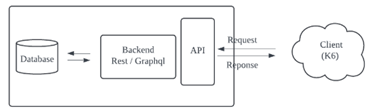
\includegraphics[width=0.6\textwidth]{assets/Picture1.png}
        \caption{Arsitektur Aplikasi}
        \label{fig:logo}
    \end{center}
\end{figure}


Server dibangun menggunakan \textbf{Node.js} dengan Hapi sebagai framework untuk \textbf{REST API} dan Graphi sebagai library untuk \textbf{GraphQL}~\cite{6}. Kedua metode \textbf{API} ini terhubung ke database PostgreSQL untuk mengambil data terkait menu. Aplikasi dideploy menggunakan layanan gratis dari \texttt{railway.com} dengan spesifikasi \textbf{2 vCPU}, \textbf{512 MB RAM}, dan \textbf{1 GB SSD Storage}. Server akan memproses permintaan yang dikirim melalui Postman, \textbf{GraphQL Playground}, atau tools K6 dan akan merespons sesuai dengan skema \textbf{API} yang digunakan.

\subsubsection{Perancangan Basis Data }

Struktur database yang digunakan untuk aplikasi ini dirancang dengan basis relasional. Terdapat empat tabel utama yang akan digunakan dalam pengelolaan data aplikasi, yaitu:

\begin{figure}[ht!]
    \begin{center}
        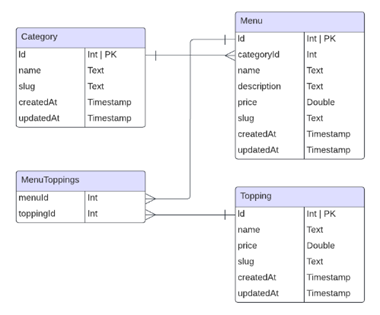
\includegraphics[width=0.6\textwidth]{assets/Picture2.png}
        \caption{Rancangan Database}
        \label{fig:logo}
    \end{center}
\end{figure}

\subsubsection{Endpoint API}

Terdapat beberapa endpoint yang dirancang untuk mengelola data menu. Setiap metode \textbf{API} \textit{(REST dan GraphQL)} memiliki cara pengelolaan endpoint yang berbeda. 

% ---------- tabellnya
\begin{table}[hbt!]
	\begin{threeparttable}
		\caption{Endpoint REST API untuk Manajemen Menu}
		\label{tabel:endpointmenu}
		 \begin{tabular}{lll}
			\toprule
			\textbf{Method} & \textbf{Endpoint} & \textbf{Keterangan} \\
			\midrule
			POST & /menu & Menambahkan menu baru \\
			GET & /menu/:id & Mengambil menu berdasarkan id \\
			PUT & /menu/:id & Memperbarui menu tertentu berdasarkan id \\
			DELETE & /menu/:id & Menghapus data menu tertentu \\
			\bottomrule
		\end{tabular}
	\end{threeparttable}
\end{table}



Berbeda dengan REST, GraphQL hanya menggunakan satu \textbf{endpoint} dengan metode \textbf{HTTP POST}, yaitu /graphql, yang digunakan untuk menangani seluruh operasi data, baik itu pengambilan, penambahan, pembaruan, maupun penghapusan data. Dalam GraphQL, struktur \textit{query} dan \textit{mutation} yang dibutuhkan untuk mengelola data, seperti kategori, menu, dan topping, didefinisikan secara eksplisit di dalam \textit{schema} GraphQL, sehingga memungkinkan klien untuk menentukan data yang diinginkan dengan lebih fleksibel dan efisien. Sebagai contoh, query untuk mengambil data menu pada GraphQL dapat ditulis seperti berikut:
 
% ---------- tabellnya
\begin{table}[hbt!]
	\begin{threeparttable}
		\caption{Operasi GraphQL API untuk Manajemen Menu}
		\label{tabel:graphqlmenu}
		 \begin{tabular}{lp{9cm}p{4.5cm}}
			\toprule
			\textbf{Operasi} & \textbf{Function} & \textbf{Remarks} \\
			\midrule
			mutation & \ { addMenu (name: "Bakso", price: 5000, categoryId: 1) \ { id, name, price \ } \ } & Menambahkan menu baru \\
			query & \{ menu (id: 1) \{ id, name, price \} \} & Mengambil menu berdasarkan id \\
			mutation & \{ updateMenu (id: 1, name: "Bakso Solo", price: 6000, categoryId: 1) \{ id, name, price \} \} & Mempengaruhi menu tertentu berdasarkan id \\
			mutation & \{ deleteMenu (id: 1) \{ id \} \} & Menghapus data menu \\
			\bottomrule
		\end{tabular}
	\end{threeparttable}
\end{table}

\subsubsection{Kebutuhan Pengujian}
Pengujian dilakukan untuk mengukur performa kedua metode \textbf{API}. Pengujian meliputi beberapa aspek, seperti:

% --------- tabellnya
\begin{table}[hbt!]
	\begin{threeparttable}
		\caption{Parameter Pengujian}
		\label{tabel:parameterpengujian}
		 \begin{tabular}{lp{10cm}}
			\toprule
			\textbf{Aspek Pengujian} & \textbf{Keterangan} \\
			\midrule
			Response Time & Waktu yang dibutuhkan untuk mengembalikan data ke client \\
			Bandwidth Usage & Jumlah total data yang diterima dan dikirim \\
			Flexibility & Kemampuan sistem dalam adaptasi terhadap berbagai kebutuhan dan perubahan yang terjadi dalam aplikasi \\
			\bottomrule
		\end{tabular}
	\end{threeparttable}
\end{table}


Parameter \textit{response time} mengukur waktu yang dibutuhkan sistem untuk memproses dan mengembalikan data ke klien. Pengujian ini dilakukan untuk mengevaluasi kecepatan dalam merespons permintaan data, yang merupakan faktor penting dalam pengalaman pengguna. Semakin cepat \textit{response time}, semakin baik kinerja aplikasi, dan semakin cepat informasi dapat disampaikan kepada pengguna. Hasil pengukuran yang optimal adalah ketika sistem mampu memberikan respons dalam waktu singkat, sedangkan hasil yang kurang baik adalah ketika waktu respons terlalu lama, yang dapat mengurangi kepuasan pengguna~\cite{7}.

Parameter \textit{bandwidth usage} mengukur efisiensi penggunaan \textit{bandwidth} jaringan dalam mentransfer data antara server dan klien. Pengujian ini bertujuan untuk mengetahui seberapa banyak sumber daya jaringan yang dibutuhkan untuk mengirimkan data. Hasil yang baik adalah ketika metode pengambilan data menggunakan \textit{bandwidth} yang efisien tanpa mengorbankan kualitas data, sedangkan hasil yang kurang baik adalah ketika penggunaan \textit{bandwidth} terlalu besar, yang dapat memperlambat proses komunikasi dan meningkatkan biaya operasional~\cite{8}.

Parameter \textit{fleksibilitas} mengacu pada kemampuan klien untuk menyesuaikan data yang dibutuhkan serta operasi \textbf{CRUD} (\textit{Create, Read, Update, Delete}). Fleksibilitas ini dibagi menjadi dua aspek utama: pertama, fleksibilitas dalam kustomisasi kebutuhan data, yang mengukur sejauh mana klien dapat menyesuaikan data yang ditampilkan sesuai dengan kebutuhannya, di mana hasil yang baik adalah hanya menampilkan data yang relevan, dan buruk jika data yang tidak diperlukan ikut ditampilkan~\cite{9}. Kedua, fleksibilitas dalam kustomisasi operasi \textbf{CRUD}, yang mengukur kemudahan klien dalam mengoperasikan seluruh operasi \textbf{CRUD} menggunakan sedikit URL; hasil yang baik adalah hanya membutuhkan satu URL untuk semua operasi, sementara hasil yang kurang baik adalah jika membutuhkan banyak URL untuk setiap operasi \textbf{CRUD}.

Pengujian ini menggunakan \textbf{K6}, sebuah \textit{tool open-source} untuk \textit{load testing} yang mampu mengukur performa \textbf{API} secara \textit{real-time}~\cite{10}. Dengan \textbf{K6}, berbagai skenario pengujian seperti waktu respon dan konsumsi \textit{bandwidth} dapat dilakukan secara sistematis~\cite{11}.


\subsubsection{Prosedur dan Pengumpulan Data}
Proses pengukuran parameter dilakukan sebagai berikut:

% ---------
\subsection*{1. Response Time}

\begin{enumerate}[label=\alph*., leftmargin=2em]
  \item Siapkan script K6 untuk REST API dan GraphQL seperti pada Koding~\ref{koding1}.

\begin{lstlisting}[language=JavaScript, caption=Koding 1. Script pengujian GraphQL dan REST API, label={koding1}, captionpos=b]
import http from 'k6/http';
import { check, sleep } from 'k6';

export let options = {
  vus: 10, // Simulasi 10 pengguna
  iterations: 200,
};

export default function () {
  // REST API
  const restRes = http.get(
    'https://api-restaurant-menu.up.railway.app/api/menu/1');
  check(restRes, { 'status is 200': (r) => r.status === 200 });

  // GraphQL
  let query = `
    query {
      menu(id: 1) {
        id
        name
      }
    }
  `;
  let headers = { 'Content-Type': 'application/json' };
  let graphqlRes = http.post(
    'https://api-restaurant-menu.up.railway.app/graphql',
    JSON.stringify({ query }),
    { headers });
  check(graphqlRes, { 'Menu status 200': (r) => r.status === 200 });
}
\end{lstlisting}


  \item Jalankan tes menggunakan K6 untuk mencatat metrik \texttt{http\_req\_duration}, yaitu durasi total setiap request.
  \item Analisis laporan K6, termasuk nilai rata-rata, minimum, median, dan maksimum dari \texttt{http\_req\_duration}.
\end{enumerate}

\vspace{1em}
\subsection*{2. Bandwidth Usage}

\begin{enumerate}[label=\alph*., leftmargin=2em]
  \item Gunakan script K6 yang sama seperti pada pengukuran response time.
  \item Jalankan tes menggunakan K6 untuk mencatat metrik \texttt{total\_bandwidth\_rest} dan \texttt{total\_bandwidth\_graphql}.
  \item Evaluasi hasil ini untuk memahami efisiensi penggunaan bandwidth oleh masing-masing metode API.
\end{enumerate}

\vspace{1em}
\subsection*{3. Flexibility}

\begin{enumerate}[label=\alph*., leftmargin=2em]
  \item Flexibility pada kebutuhan data diuji dengan mengirim permintaan ke REST API atau GraphQL untuk mendapatkan data tertentu menggunakan Postman.
  \item Fleksibilitas Kustomisasi Operasi CRUD (Create, Read, Update, Delete):\\
  Pertama, fleksibilitas dalam menyesuaikan kebutuhan data melalui input query dan data menu seperti \texttt{name}, \texttt{price}, \texttt{categoryId}.\\
  Kedua, kemudahan bagi klien untuk menjalankan seluruh operasi CRUD menggunakan sedikit URL, baik melalui REST API maupun GraphQL.
\end{enumerate}

Pengujian dilakukan pada beberapa \textit{endpoint} \textbf{REST API} dan \textbf{query} GraphQL yang akan memanipulasi data menu pada aplikasi restoran. Untuk \textbg{REST API}, pengambilan data dilakukan dengan beberapa permintaan, sedangkan untuk GraphQL, hanya satu permintaan diperlukan untuk mengambil semua data yang relevan ~\cite{12}. Data hasil pengujian akan dikumpulkan dan dianalisis untuk melihat perbedaan metode REST API dan GraphQL. 

%%%%%%%%%%%%%%%%%%%%%%%%%%%%%%%%%%%%%%%%%% HASIL %%%%%%%%%%%%%%%%%%%%%%%%%%%%
\section{Hasil dan Pembahasan}

\subsection{Parameter Response Time dan Bandwidth Usage}

Pada bagian ini menyajikan hasil pengukuran dan analisis performa terhadap parameter \textit{response time} dan \textit{bandwidth usage} yang telah diimplementasikan. Pengujian dilakukan menggunakan \texttt{K6} untuk membandingkan performa masing-masing metode. Iterasi 100 dipilih untuk memastikan data \textit{response time} dan \textit{bandwidth usage} stabil dan representatif. Jumlah ini cukup sesuai karena memenuhi konsistensi data, memadai terutama untuk menghindari \textit{outlier} atau fluktuasi data yang terjadi dalam pengujian tunggal. Iterasi yang terlalu banyak bisa memakan waktu dan sumber daya lebih besar, sehingga iterasi tersebut menjadi kompromi antara akurasi data dan efisiensi proses pengujian~\cite{13}. 

Tolok ukur yang digunakan adalah kecepatan respons, dengan metode yang lebih cepat dianggap lebih baik. Selain itu, \textit{bandwidth usage} dianalisis untuk mengukur efisiensi data yang dikirim. \textit{Bandwidth usage} yang rendah menunjukkan efisiensi yang baik, sementara penggunaan yang tinggi dapat memperlambat aplikasi dan meningkatkan beban jaringan.

\subsubsection{Hasil Pengujian Skenario GET}


\noindent
\begin{minipage}{0.48\textwidth}
    \begin{figure}[H]
        \centering
        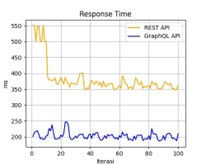
\includegraphics[width=\textwidth]{assets/Picture3.jpg}
        \caption{Arsitektur Aplikasi}
        \label{fig:arsitektur}
    \end{figure}
\end{minipage}%
\hspace{0.04\textwidth}
\begin{minipage}{0.48\textwidth}
    \begin{figure}[H]
        \centering
        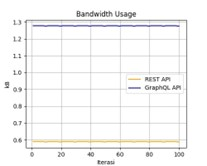
\includegraphics[width=\textwidth]{assets/Picture4.jpg}
        \caption{Diagram Alur}
        \label{fig:diagram}
    \end{figure}
\end{minipage}




% \begin{figure}[ht!]
%     \centering
%     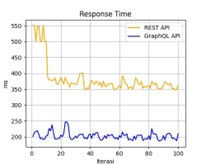
\includegraphics[width=0.8\textwidth]{assets/Picture3.jpg}  
%     \caption{Arsitektur Aplikasi}  % Caption untuk gambar pertama
%     \label{fig:arsitektur}
% \end{figure}

% \begin{figure}[ht!]
%     \centering
%     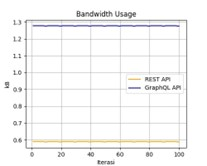
\includegraphics[width=0.8\textwidth]{assets/Picture4.jpg}  
%     \caption{Diagram Alur}  % Caption untuk gambar kedua
%     \label{fig:diagram}
% \end{figure}



Merujuk pada Gambar 3-4, pengujian\textit{response time} \textbf{REST API} menunjukkan waktu respons yang lebih tinggi dan fluktuatif di awal sebelum stabil, sedangkan GraphQL lebih konsisten dan cepat, menunjukkan efisiensi GraphQL dalam memproses permintaan GET. Namun, pada penggunaan \textit{bandwidth}, GraphQL menggunakan \textit{bandwidth} sedikit tinggi daripada REST API.

\subsubsection{Hasil Pengujian Skenario POST}

\noindent
\begin{minipage}{0.48\textwidth}
    \begin{figure}[H]
        \centering
        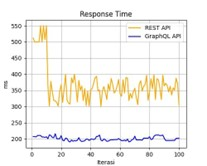
\includegraphics[width=\textwidth]{assets/Picture5.jpg}
        \caption{Arsitektur Aplikasi}
        \label{fig:arsitektur}
    \end{figure}
\end{minipage}%
\hspace{0.04\textwidth}
\begin{minipage}{0.48\textwidth}
    \begin{figure}[H]
        \centering
        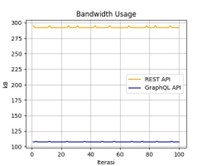
\includegraphics[width=\textwidth]{assets/Picture6.jpg}
        \caption{Diagram Alur}
        \label{fig:diagram}
    \end{figure}
\end{minipage}



Merujuk pada Gambar~\ref{gambar5-6}, pengujian \textit{POST} menunjukkan bahwa GraphQL memiliki waktu respons yang lebih rendah dan konsisten dibandingkan dengan REST API yang cenderung fluktuatif dan lebih lambat. Sementara itu, dari segi penggunaan \textit{bandwidth}, REST API tercatat menggunakan \textit{bandwidth} yang lebih tinggi, sedangkan GraphQL lebih efisien dalam mentransfer data, menunjukkan keunggulan dalam efisiensi komunikasi jaringan.

\subsubsection{Hasil Pengujian Skenario PUT}

\noindent
\begin{minipage}{0.48\textwidth}
    \begin{figure}[H]
        \centering
        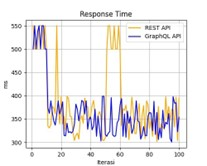
\includegraphics[width=\textwidth]{assets/Picture7.jpg}
        \caption{Arsitektur Aplikasi}
        \label{fig:arsitektur}
    \end{figure}
\end{minipage}%
\hspace{0.04\textwidth}
\begin{minipage}{0.48\textwidth}
    \begin{figure}[H]
        \centering
        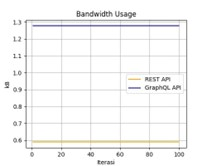
\includegraphics[width=\textwidth]{assets/Picture8.jpg}
        \caption{Diagram Alur}
        \label{fig:diagram}
    \end{figure}
\end{minipage}

Merujuk pada Gambar~\ref{gambar7-8}, hasil pengujian pada skenario \textit{PUT} menunjukkan bahwa waktu respons untuk REST API dan GraphQL cenderung fluktuatif namun relatif setara. Hal ini mengindikasikan bahwa keduanya mampu menangani permintaan \textit{update} data dengan performa yang serupa dalam hal kecepatan.

Namun, dalam hal penggunaan \textit{bandwidth}, GraphQL menunjukkan konsumsi yang lebih tinggi dibandingkan REST API. Hal ini menunjukkan bahwa REST API lebih hemat dalam penggunaan \textit{bandwidth} pada operasi \textit{PUT}, kemungkinan disebabkan oleh struktur permintaan yang lebih sederhana atau data yang dikirimkan lebih ringkas. Perbedaan ini perlu dipertimbangkan ketika efisiensi jaringan menjadi faktor utama dalam pengembangan aplikasi.


\subsubsection{Hasil Pengujian Skenario DELETE}

\noindent
\begin{minipage}{0.48\textwidth}
    \begin{figure}[H]
        \centering
        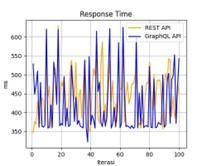
\includegraphics[width=\textwidth]{assets/Picture9.jpg}
        \caption{Arsitektur Aplikasi}
        \label{fig:arsitektur}
    \end{figure}
\end{minipage}%
\hspace{0.04\textwidth}
\begin{minipage}{0.48\textwidth}
    \begin{figure}[H]
        \centering
        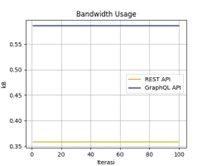
\includegraphics[width=\textwidth]{assets/Picture10.jpg}
        \caption{Diagram Alur}
        \label{fig:diagram}
    \end{figure}
\end{minipage}

Merujuk pada Gambar \ref{gambar9-10}, hasil temuan menunjukkan bahwa GraphQL dan REST API sama-sama unggul dalam hal skalabilitas untuk permintaan yang tinggi. Namun, GraphQL lebih efisien dalam penggunaan \textit{bandwidth} karena kemampuannya menghindari \textit{over-fetching} \cite{14,15}. Pada skenario pengujian \textit{GET}, \textit{PUT}, dan \textit{DELETE}, perbedaan performa antara kedua arsitektur tidak terlalu signifikan, namun GraphQL tetap menunjukkan keunggulan dibandingkan REST API dari segi efisiensi dan konsistensi performa.

GraphQL menunjukkan efektivitas yang tinggi dalam mengurangi waktu respons, sebagaimana terlihat dari rata-rata waktu respons yang cepat serta distribusi data yang stabil. Dengan kemampuannya memfasilitasi permintaan data yang lebih spesifik, GraphQL hanya mengirimkan data yang dibutuhkan oleh klien. Hal ini berbeda dengan REST API yang sering mengirimkan data secara berlebih dalam satu respons. Pendekatan ini menjadikan GraphQL ideal untuk aplikasi yang membutuhkan performa tinggi, khususnya dalam lingkungan dengan kebutuhan data kompleks namun spesifik. Selain itu, penggunaan \textit{bandwidth} pada GraphQL terbukti lebih efisien, sesuai dengan karakternya yang menghindari pengiriman data yang tidak diperlukan sehingga mampu mengurangi \textit{overhead} komunikasi \cite{16}. Meskipun REST API menunjukkan kinerja yang baik dalam skala besar, GraphQL memiliki keunggulan signifikan dalam efisiensi penggunaan \textit{bandwidth} referensi \cite{17}.
% -----------------------------
%  = = = = = = = = = = = =  TEST 
% \textbf{TEST aja} 
% - \cite{article}
% - \cite{articleLekshmi}
% - \cite{desperindagkaltim}
% - \cite{Erwi2015}
% - \cite{George1999}
% - \cite{Growth2009}
% - \cite{Kolodzy}
% - \cite{Wu}
% - \cite{Vygotsky1999}
% - \cite{Transport}
% - \cite{soil-1-273-2015}
% - \cite{Setyowati2020}
% - \cite{Rikie}
% - \cite{Pramana2013}
% = \cite{Lutfiyana2017}
% - \cite{Kolodzy}
% - \cite{Johnson1962}
% - \cite{Lutfiyana2017}



\subsection{Parameter Flexibility}

\subsubsection{Hasil Pengujian Fleksibilitas Kustomisasi Kebutuhan Data}

Hasil query dianalisis berdasarkan fleksibilitas metode dalam menyesuaikan data sesuai kebutuhan klien melalui operasi \textit{read} di Postman. Suatu metode dinilai baik apabila mampu menyajikan data relevan sesuai permintaan, sedangkan metode yang menampilkan data berlebihan atau tidak diperlukan dianggap kurang fleksibel. Hasil pengujian sebagai berikut:

\paragraph{a. Implementasi Fleksibilitas Klien REST API}

\begin{table}[hbt!]
  \begin{threeparttable}
    \caption{Fleksibilitas Klien REST API}
    \label{tabel:restapi-flex}
    \begin{tabular}{lp{9cm}}
      \toprule
      \textbf{Kebutuhan} & \textbf{Hasil Operasi} \\
      \midrule
      Menampilkan data: id, name & \{ "id": 7, "name": "Bakso Sony", "price": 10000, "createdAt": "2025-01-05T11:20:29.376Z", "categoryId": 1 \} \\
      Menampilkan data: id, name, price & \{ "id": 7, "name": "Bakso Sony", "price": 10000, "createdAt": "2025-01-05T11:20:29.376Z", "categoryId": 1 \} \\
      \bottomrule
    \end{tabular}
  \end{threeparttable}
\end{table}


Tabel~\ref{tabel:restapi-flex} menunjukkan bahwa REST API tidak mendukung kustomisasi data secara spesifik. Sebagai contoh, meskipun klien hanya memerlukan \texttt{id} dan \texttt{name}, REST API tetap menampilkan seluruh data, termasuk \texttt{price}, \texttt{createdAt}, dan \texttt{categoryId} yang tidak diminta secara eksplisit.

\paragraph{b. Implementasi Dengan Parameter Fleksibilitas Klien GraphQL}

\begin{table}[hbt!]
  \begin{threeparttable}
    \caption{Fleksibilitas Klien GraphQL}
    \label{tabel:graphql-flex}
    \begin{tabular}{lp{9cm}}
      \toprule
      \textbf{Kebutuhan} & \textbf{Hasil Operasi} \\
      \midrule
      Menampilkan data: id, name & Query: \texttt{\{ menu(id:7) \{ id name \} \}} \newline Hasil: \{ "id": 7, "name": "Bakso Sony" \} \\
      Menampilkan data: id, name, price & Query: \texttt{\{ menu(id:7) \{ id name price \} \}} \newline Hasil: \{ "id": 7, "name": "Bakso Sony", "price": 10000 \} \\
      \bottomrule
    \end{tabular}
  \end{threeparttable}
\end{table}


GraphQL mendukung kustomisasi data sesuai kebutuhan klien, hanya menampilkan informasi yang diminta seperti ditunjukkan pada Tabel~\ref{tabel:graphql-flex}. Ini menjadikan GraphQL lebih fleksibel dan efisien karena tidak menyertakan informasi yang tidak relevan.

\subsubsection{Hasil Pengujian Fleksibilitas Kustomisasi Operasi CRUD}

Bagian ini menyajikan hasil perbandingan yang telah diimplementasikan berdasarkan fleksibilitas dalam melakukan kustomisasi operasi CRUD oleh klien.

\begin{table}[hbt!]
  \begin{threeparttable}
    \caption{Jumlah URL pada Operasi CRUD}
    \label{tabel:crud-url}
    \begin{tabular}{lp{9cm}}
      \toprule
      \textbf{Metode} & \textbf{URL} \\
      \midrule
      REST API & 
      POST \url{https://api-restaurant-menu.up.railway.app/api/menu} \newline
      GET \url{https://api-restaurant-menu.up.railway.app/api/menu/:id} \newline
      PUT \url{https://api-restaurant-menu.up.railway.app/api/menu/:id} \newline
      DELETE \url{https://api-restaurant-menu.up.railway.app/api/menu/:id} \\
      \midrule
      GraphQL & POST \url{https://api-restaurant-menu.up.railway.app/graphql} \\
      \bottomrule
    \end{tabular}
  \end{threeparttable}
\end{table}


Berdasarkan Tabel~\ref{tabel:crud-url}, GraphQL hanya memerlukan satu URL untuk menjalankan seluruh operasi CRUD, sedangkan REST API membutuhkan URL berbeda untuk tiap operasinya. Hal ini menunjukkan bahwa GraphQL lebih fleksibel dalam hal kustomisasi, memungkinkan klien untuk mengelola berbagai operasi hanya dari satu endpoint. Sebaliknya, REST API kurang mendukung fleksibilitas serupa karena ketergantungannya pada struktur URL yang berbeda-beda.


%%%%%%%%%%%%%%%%%%%%%%%%%%%%%%%%%%%%%PEMBAHASAN %%%%%%%%%%%%%%%%%%%%%




%%%%%%%%%%%%%%%%%%%%%%%%%%%%%%%%%%% SIMPULAN %%%%%%%%%%%%%%%%%%%%%%%%%
\section{Simpulan}

Hasil pengujian yang telah dilakukan berdasarkan skenario yang telah disusun menghasilkan beberapa kesimpulan sebagai berikut:

\begin{enumerate}[left=0.5in]
    \item \textbf{Skenario Pengujian GET:} Arsitektur GraphQL API menunjukkan perbedaan performa yang cukup signifikan dibandingkan dengan REST API saat menggunakan lingkungan cloud. Selain mampu mengatasi beberapa kelemahan REST API, GraphQL API juga mampu bersaing dari segi performa. Pada skenario pengujian POST, PUT, dan DELETE, meskipun perbedaan performa antara kedua arsitektur tidak terlalu signifikan, GraphQL API tetap menunjukkan performa yang lebih baik dibandingkan REST API.
    \item \textbf{Penggunaan Bandwidth:} Penggunaan Bandwidth menunjukkan bahwa GraphQL lebih efisien dibandingkan REST API. GraphQL hanya mengirim dan menerima data yang dibutuhkan, sementara REST API cenderung mengirimkan data berlebih yang tidak selalu diperlukan oleh klien. Efisiensi bandwidth ini menjadikan GraphQL lebih hemat dalam penggunaan data dan lebih cepat dalam kondisi jaringan terbatas.
    \item \textbf{Fleksibilitas:} Metode GraphQL sangat fleksibel karena dapat mengizinkan klien untuk kustomisasi terhadap kebutuhan data sehingga nantinya data yang ditampilkan ke klien akan sesuai dengan permintaan atau kebutuhan klien, sedangkan metode REST API tidak dapat melakukan hal yang dilakukan GraphQL karena REST API tidak dapat mengizinkan klien untuk kustomisasi terhadap kebutuhan data.
\end{enumerate}

Adapun kekurangan yang masih ada dalam penelitian ini, penulis memberikan beberapa rekomendasi untuk penelitian selanjutnya sebagai berikut:

\begin{enumerate}[left=0.5in]
    \item \textbf{Penggunaan Layanan Cloud Berbayar:} Penelitian ini dilakukan dalam lingkungan cloud dengan memanfaatkan layanan gratis. Penelitian selanjutnya disarankan menggunakan layanan cloud berbayar dengan spesifikasi yang lebih tinggi. Hal ini bertujuan untuk mengevaluasi apakah peningkatan sumber daya infrastruktur, seperti CPU, RAM, dan bandwidth, memiliki dampak signifikan terhadap performa arsitektur GraphQL API dan REST API.
    \item \textbf{Penambahan Parameter Uji:} Penelitian selanjutnya diharapkan dapat menambahkan parameter uji lain seperti latency, throughput, atau standar deviasi untuk mendapatkan analisis yang lebih komprehensif.
\end{enumerate}

%%%%%%%%%%%%%%%%%%%%%%%%%%%%%%%%%%% PUSTAKA %%%%%%%%%%%%%%%%%%%%%%%%%%%%%%%
\section*{Ucapan Terima kasih}
Dengan penuh rasa syukur kepada Allah SWT atas rahmat, hidayah, dan karunia-Nya, penelitian ini berhasil diselesaikan dengan baik. Penulis juga menyampaikan terima kasih yang sebesar-besarnya kepada semua pihak yang telah memberikan dukungan, saran, serta bantuan selama proses penelitian ini hingga dapat terselesaikan.

\renewcommand{\refname}{Pustaka} %%% nonaktifkan bila artikel bahasa inggris
	\bibliographystyle{IEEEtran}
\bibliography{reference}
% ---------- Manual daftar pusrtaka
\end{document}
